% anhang.tex
\chapter{Visualisierung der Dürrfleckenkrankheit}
\label{anahngb}
\begin{figure}[h!]
	\centering
	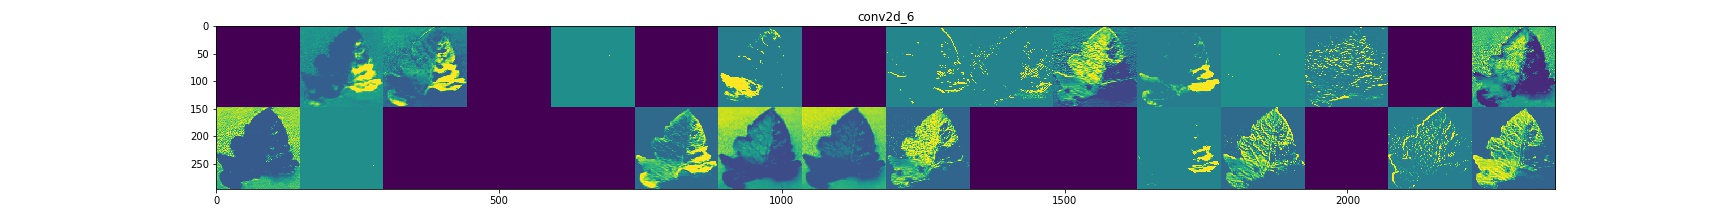
\includegraphics[width=\textwidth]{visualisierungen/early/activation/early0.JPG}
	\caption{Visualisierung der Aktivierungswerte in der ersten Faltungschicht von der Dürrfleckenkrankheit (eigene Darstellung).}
	\label{}
\end{figure}

\begin{figure}[h!]
	\centering
	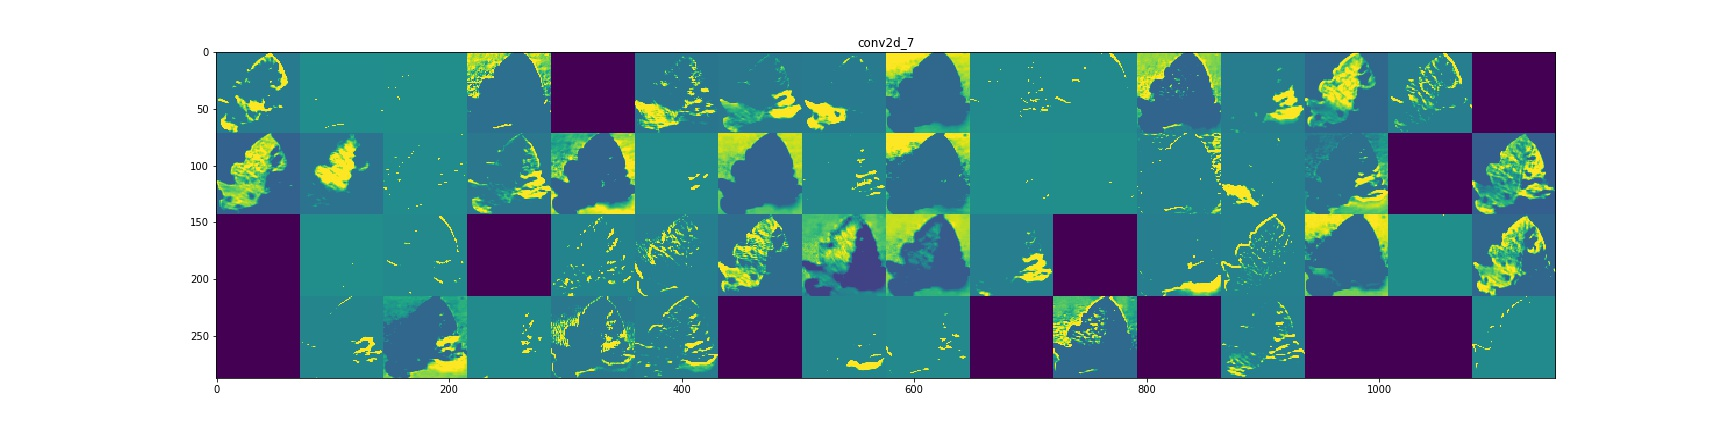
\includegraphics[width=\textwidth]{visualisierungen/early/activation/early3.JPG}
	\caption{Visualisierung der Aktivierungswerte in der zweiten Faltungschicht von der Dürrfleckenkrankheit (eigene Darstellung).}
	\label{}
\end{figure}

\begin{figure}[h!]
	\centering
	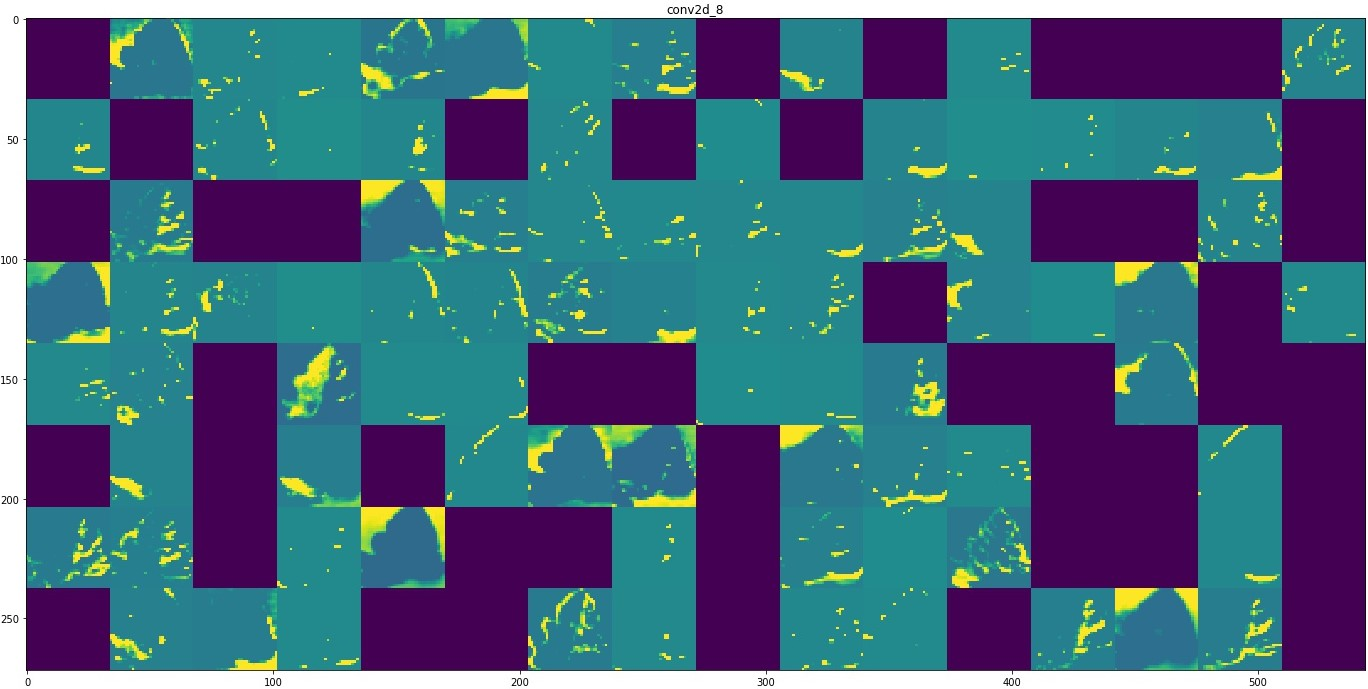
\includegraphics[width=\textwidth]{visualisierungen/early/activation/early6.JPG}
	\caption{Visualisierung der Aktivierungswerte in der dritten Faltungschicht von der Dürrfleckenkrankheit (eigene Darstellung).}
	\label{}
\end{figure}

\begin{figure}[h!]
	\centering
	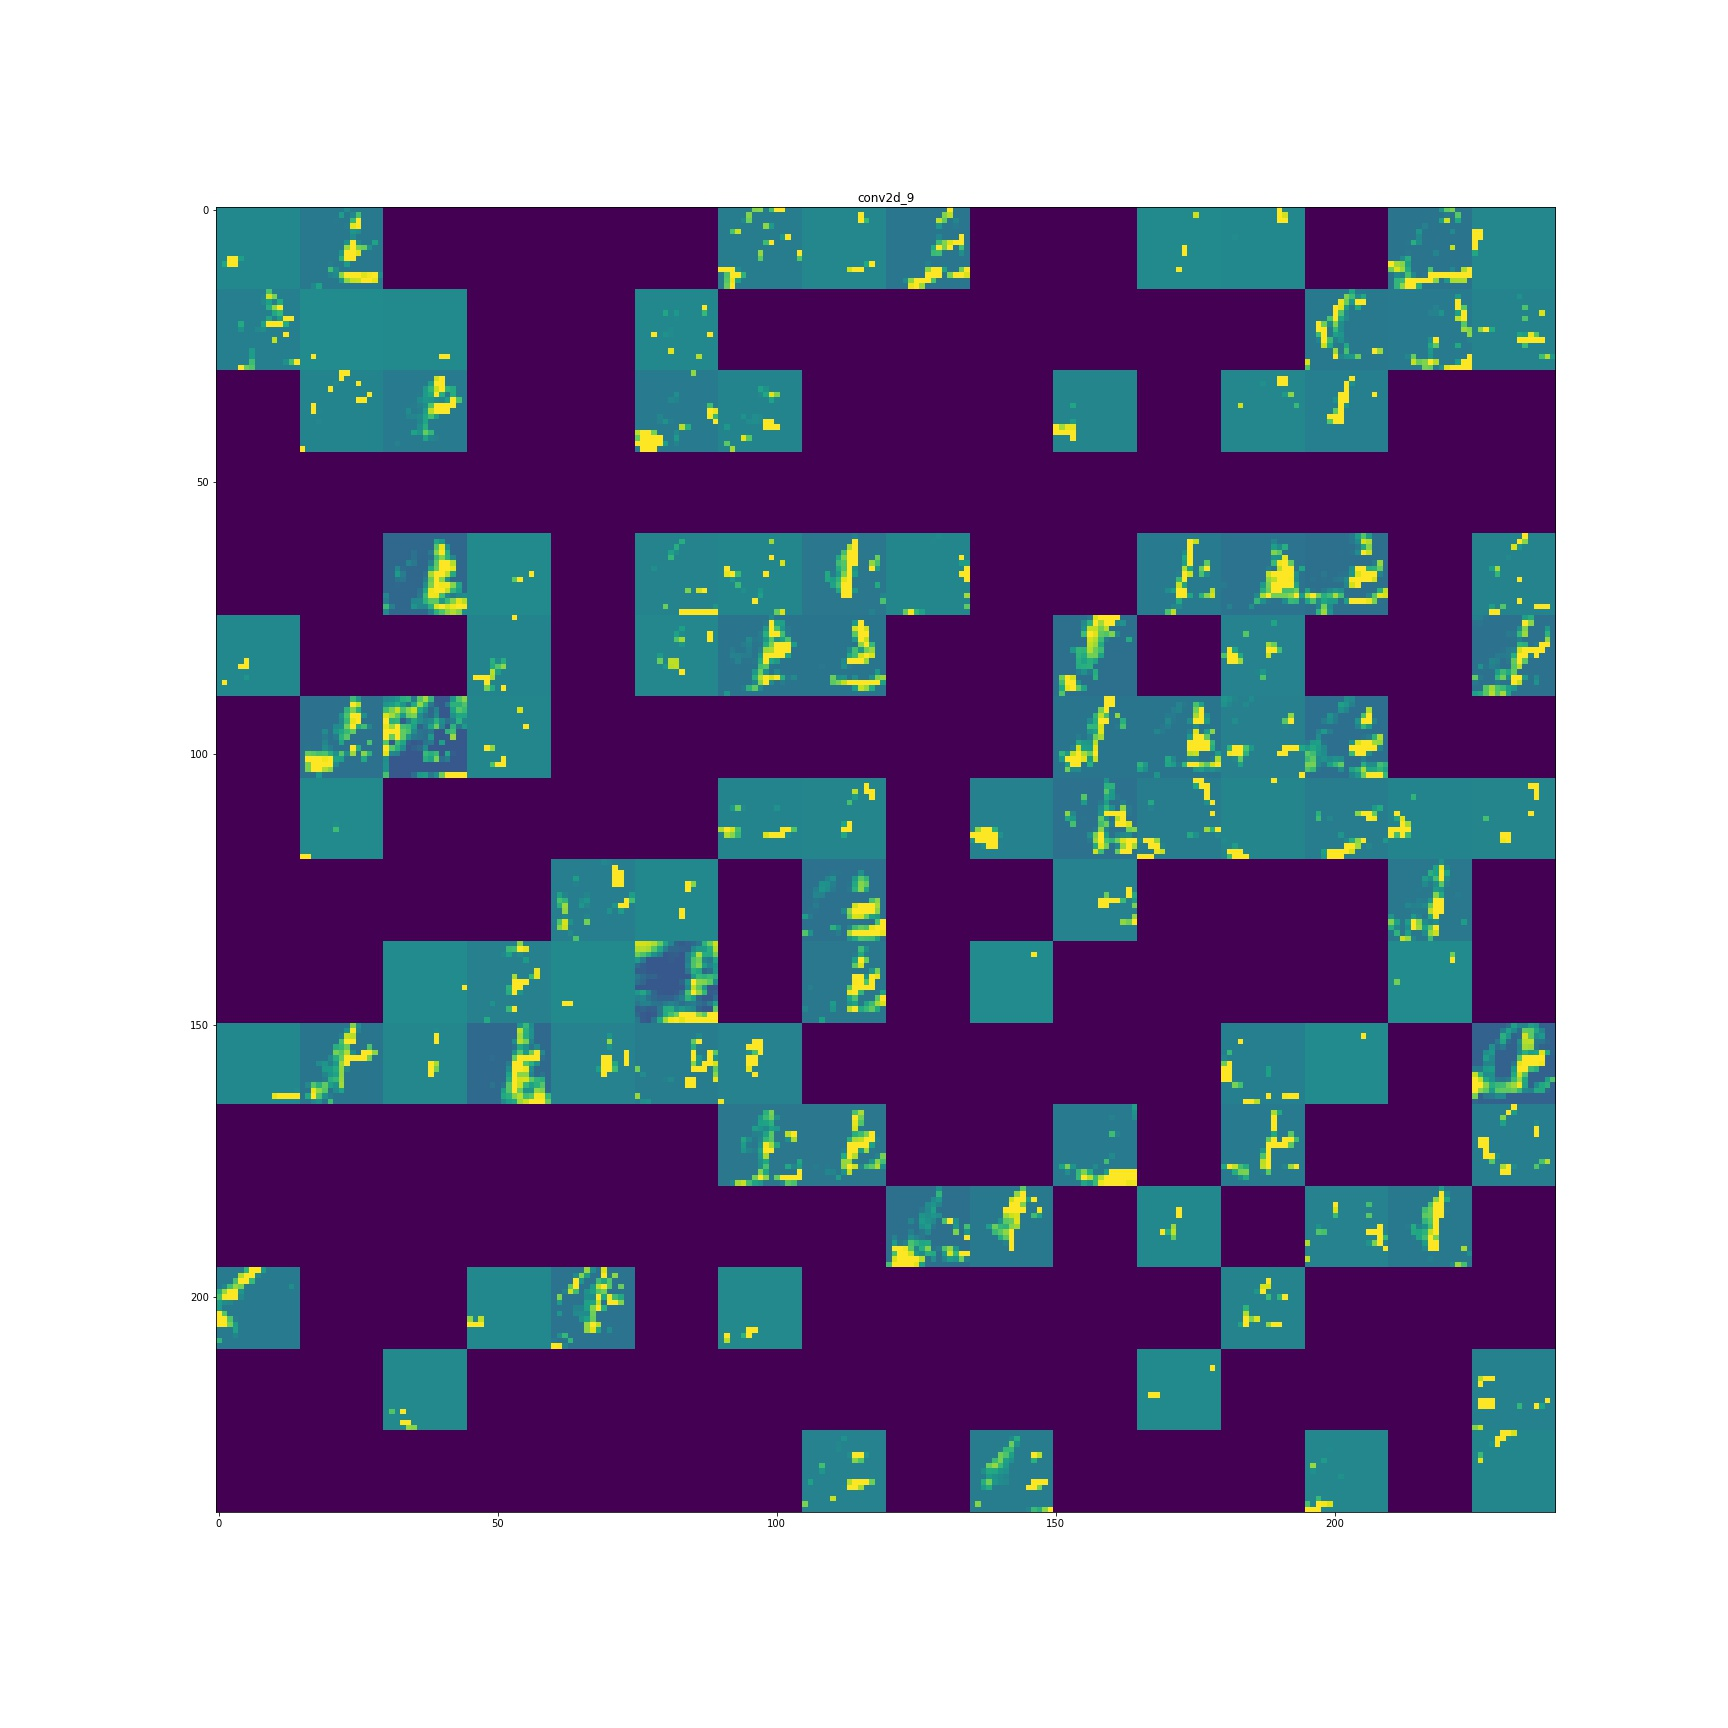
\includegraphics[width=\textwidth]{visualisierungen/early/activation/early8.JPG}
	\caption{Visualisierung der Aktivierungswerte in der vierten Faltungschicht von der Dürrfleckenkrankheit (eigene Darstellung).}
	\label{early8_anhang}
\end{figure}

\begin{figure}[h!]
	\centering
	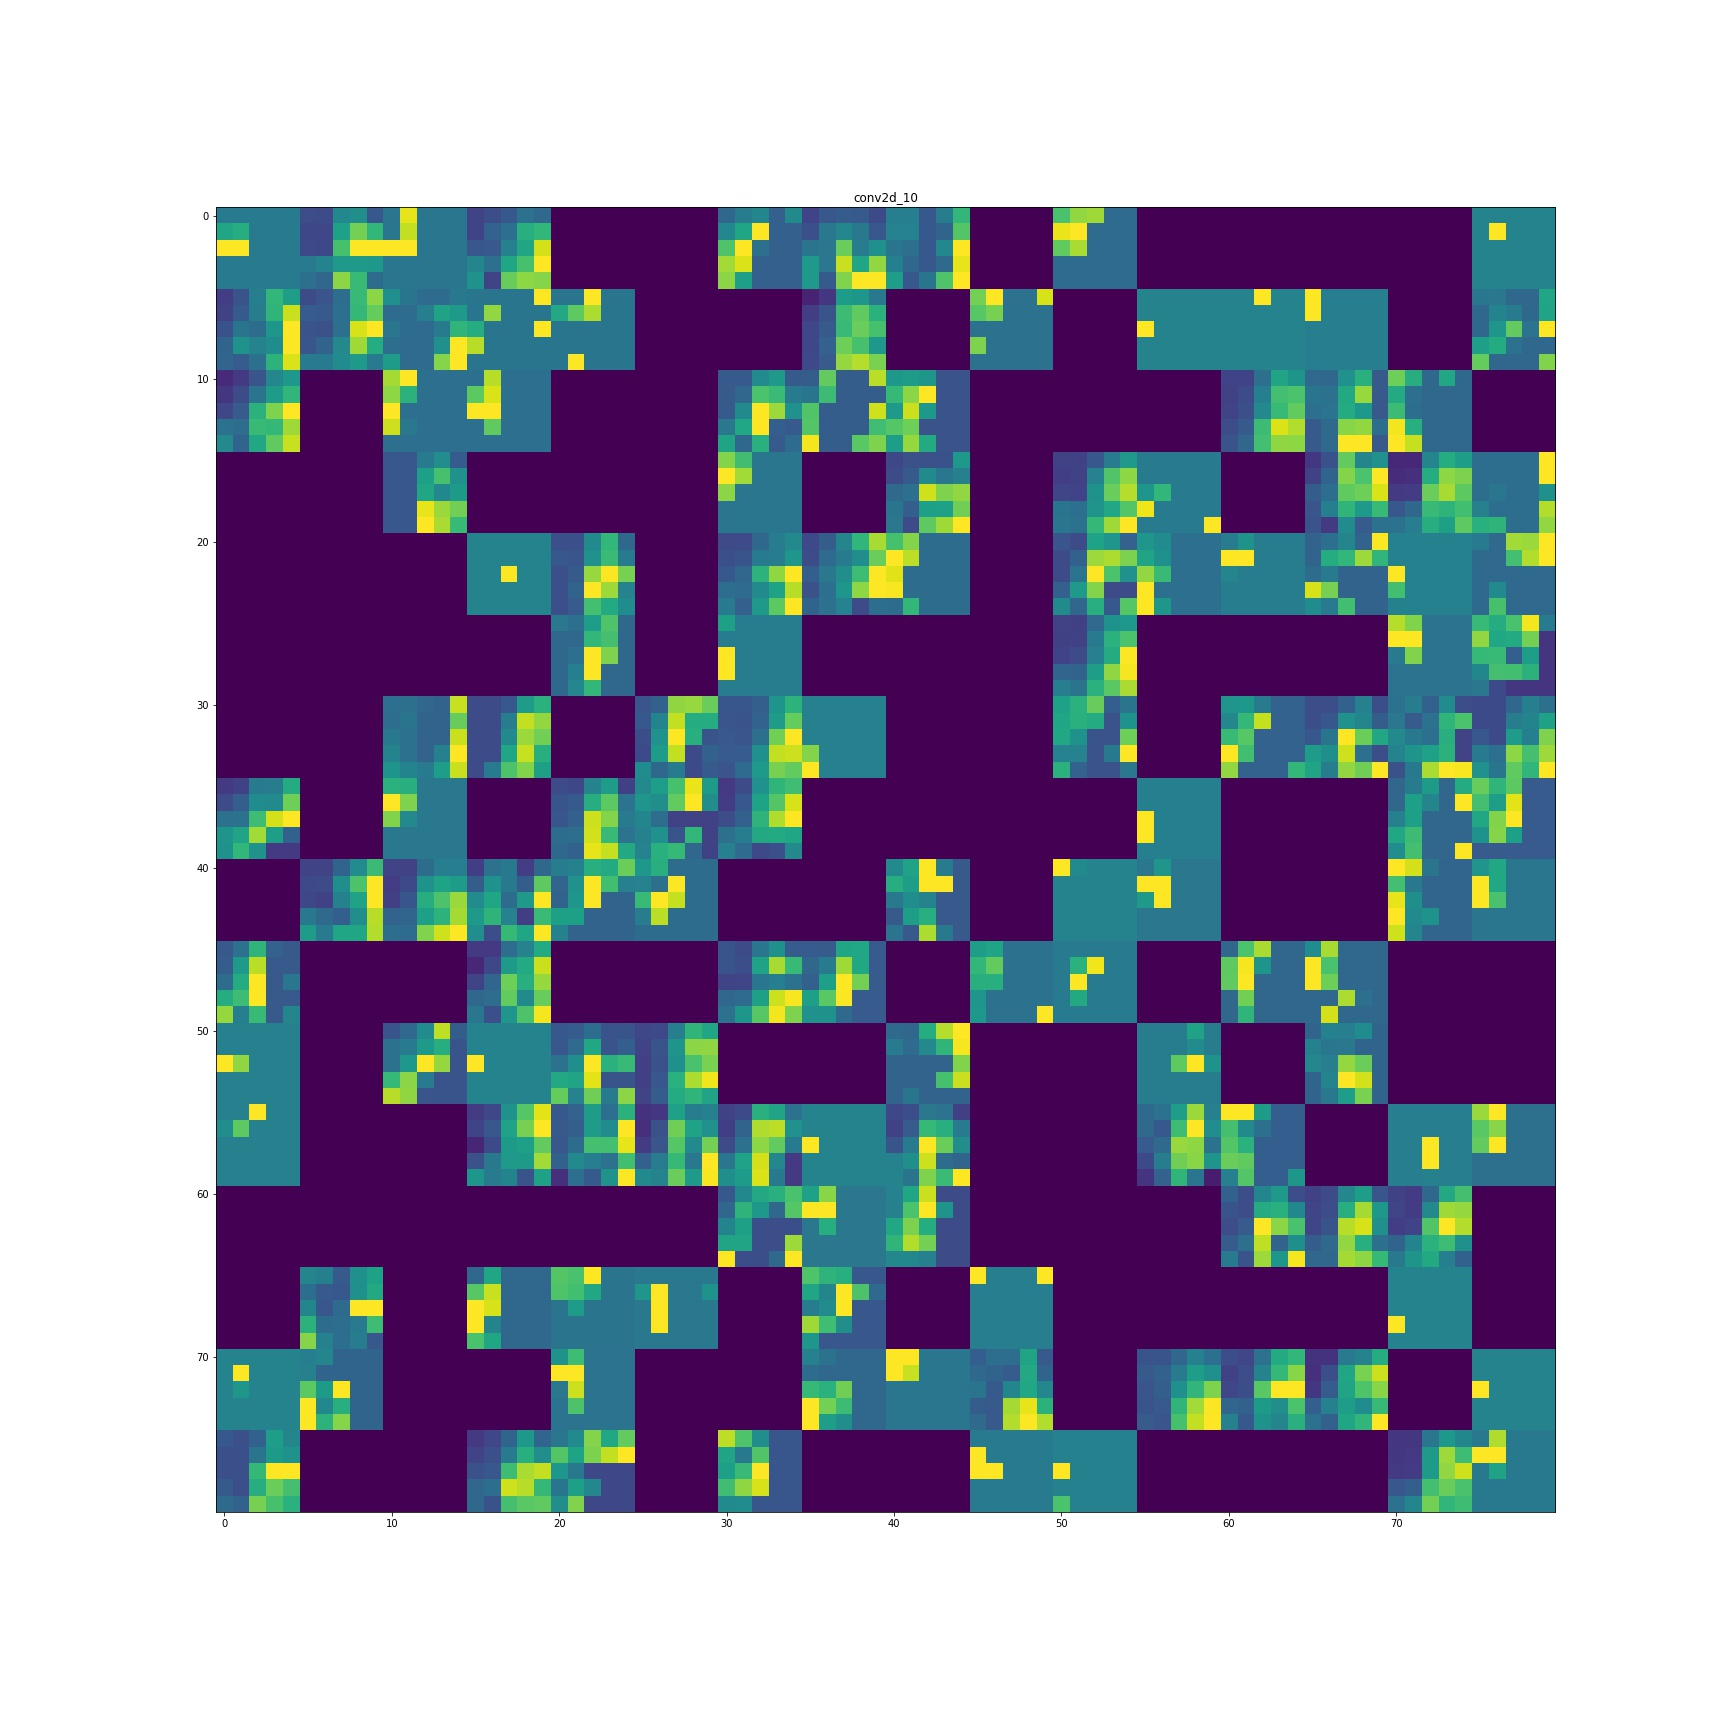
\includegraphics[width=\textwidth]{visualisierungen/early/activation/early10.JPG}
	\caption{Visualisierung der Aktivierungswerte in der fünften Faltungschicht von der Dürrfleckenkrankheit (eigene Darstellung).}
	\label{}
\end{figure}

%%%%%%%%%%%%%%%%%%%%%%%%%%%%%%%%%%%%%%%%%%%%%%%%%%%%%%%%%%

\begin{figure}[h!]
	\centering
	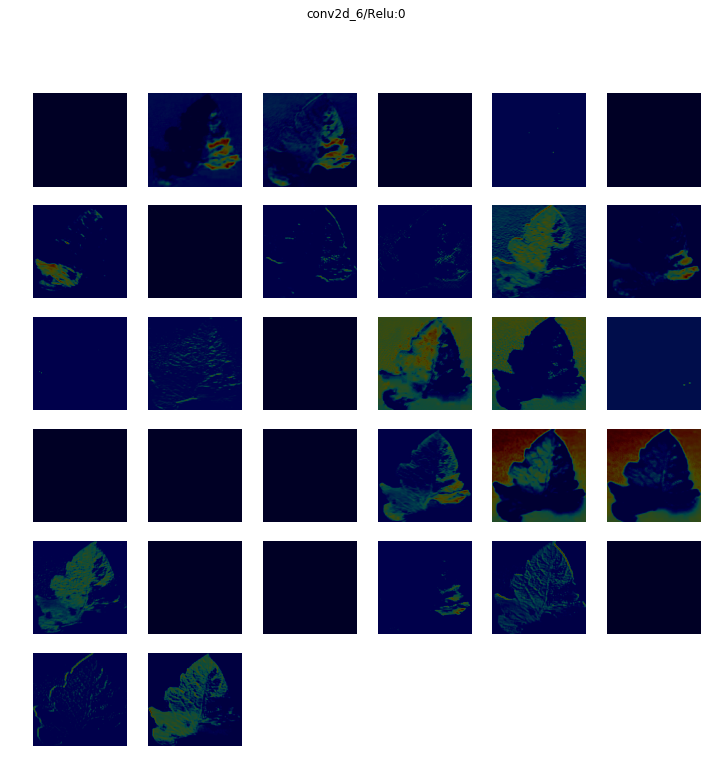
\includegraphics[width=\textwidth]{visualisierungen/early/heatmap_mit/conv2d_6.png}
	\caption{Visualisierung der Aktivierungswerte als Heatmap in der ersten Faltungschicht von der Dürrfleckenkrankheit (eigene Darstellung).}
	\label{}
\end{figure}

\begin{figure}[h!]
	\centering
	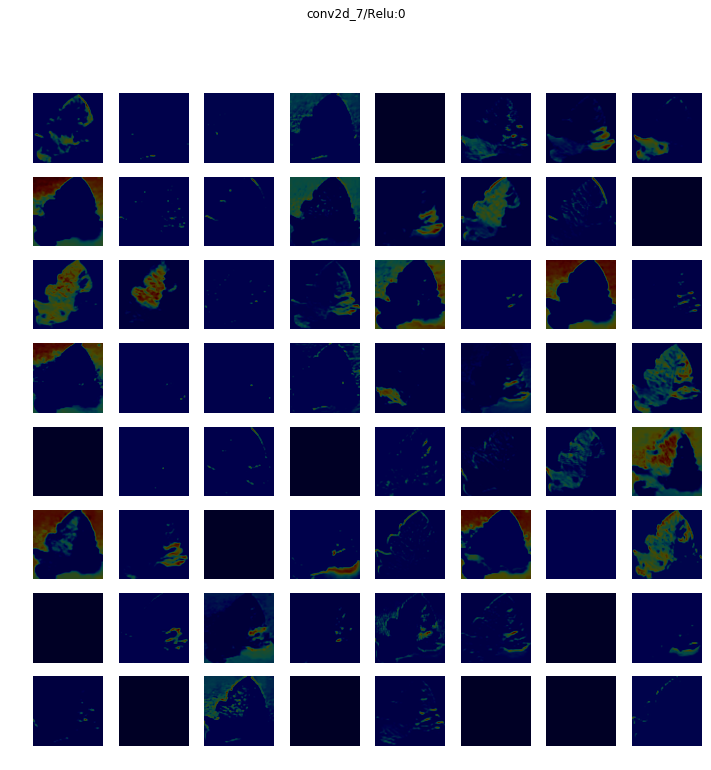
\includegraphics[width=\textwidth]{visualisierungen/early/heatmap_mit/conv2d_7.png}
	\caption{Visualisierung der Aktivierungswerte als Heatmap in der zweiten Faltungschicht von der Dürrfleckenkrankheit (eigene Darstellung).}
	\label{}
\end{figure}

\begin{figure}[h!]
	\centering
	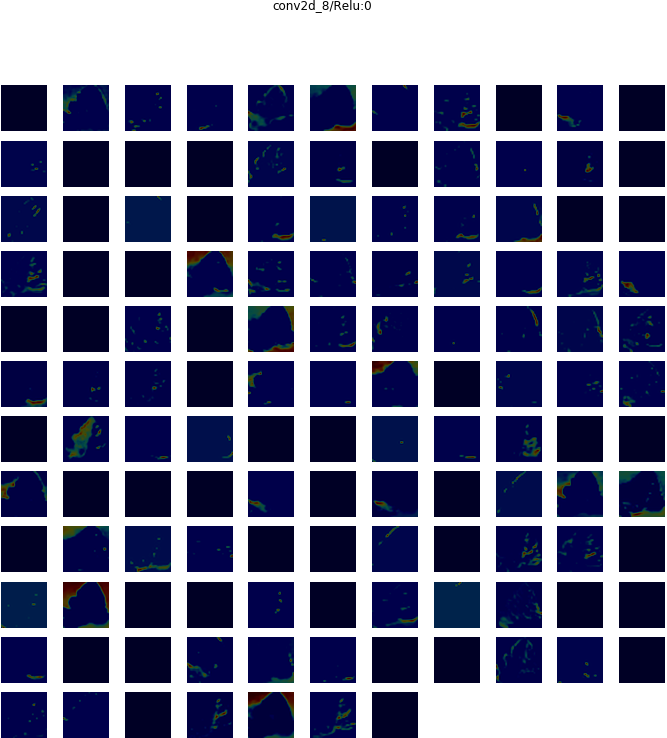
\includegraphics[width=\textwidth]{visualisierungen/early/heatmap_mit/conv2d_8.png}
	\caption{Visualisierung der Aktivierungswerte als Heatmap in der dritten Faltungschicht von der Dürrfleckenkrankheit (eigene Darstellung).}
	\label{}
\end{figure}

\begin{figure}[h!]
	\centering
	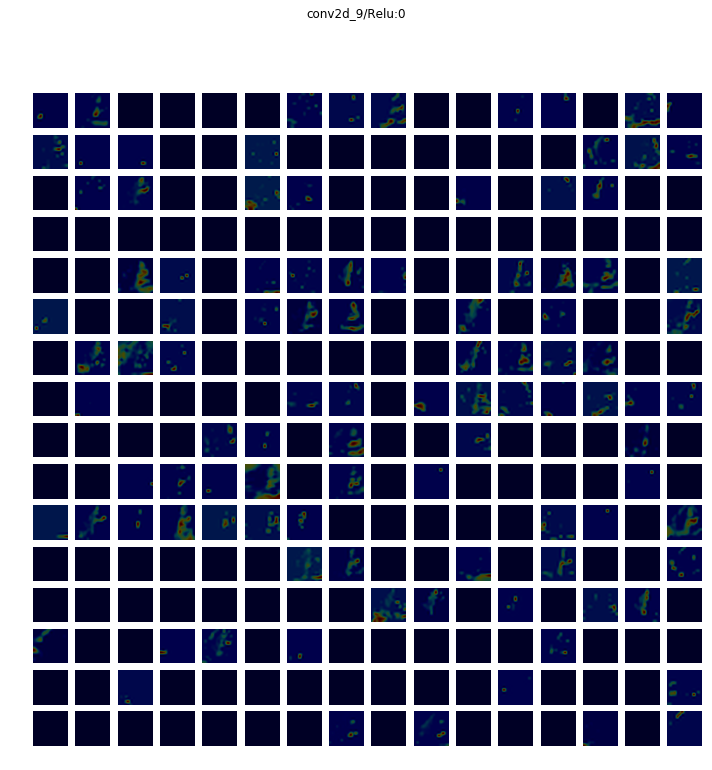
\includegraphics[width=\textwidth]{visualisierungen/early/heatmap_mit/conv2d_9.png}
	\caption{Visualisierung der Aktivierungswerte als Heatmap in der vierten Faltungschicht von der Dürrfleckenkrankheit (eigene Darstellung).}
	\label{conv2d_9_anhang}
\end{figure}

\begin{figure}[h!]
	\centering
	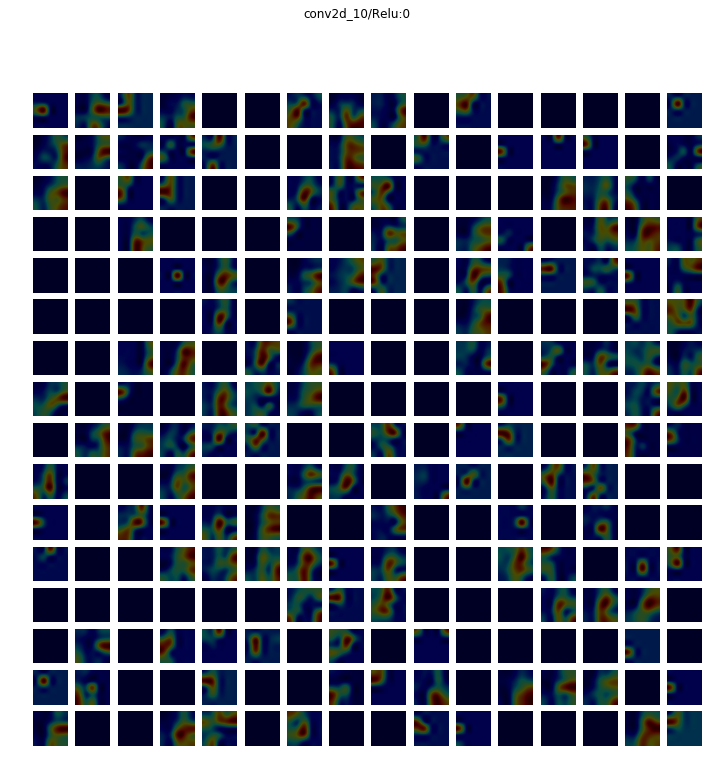
\includegraphics[width=\textwidth]{visualisierungen/early/heatmap_mit/conv2d_10.png}
	\caption{Visualisierung der Aktivierungswerte als Heatmap in der fünften Faltungschicht von der Dürrfleckenkrankheit (eigene Darstellung).}
	\label{}
\end{figure}